\documentclass[10pt, red]{beamer}
\usetheme{JuanLesPins}
\usepackage[english]{babel}
\usepackage[latin1]{inputenc} 
\setbeamercovered{transparent}


\title[CUDAQCADesigner]{A Parallel Version of the MiNa's Quantum Dot Cellular Automata IDE - QCADesigner}

\author{Riccardo Cattaneo, Giuseppe Chindemi}

\institute{
  Politecnico di Milano\\
  HPPS
}

\date{June 22 2010}

\pgfdeclareimage[height=0.5cm]{logo}{img/polimi}
\logo{\pgfuseimage{logo}}


\begin{document}

\begin{frame}
  \titlepage
\end{frame}

\section{Introduction}
	\begin{frame}{Why?}
		\begin{itemize} 
			\item Si based technology is reaching its physical limits due to aggressive miniaturization, progressively increasing packaging densities, clock distribution and dissipation issues
			\item Alternatives are being studied right now in order to overcome these limits (different technologies)
			\item QCA cells are one of these
<<<<<<< .mine
			\item QCADesigner is the most mature tool for layouting and simulating QCA cells based circuits
			\item QCADesigner is unreasonably slow to simulate more bigger-than-toy circuits
=======
			\item QCADesigner is the most mature tool for layouting and simulating QCA cells based circuits, yet, in the original implementation it is unreasonably slow to simulate more bigger-than-toy ones
			\item Exploitation of other approach in order to obtain significant speedups
>>>>>>> .r547
		\end{itemize}
	\end{frame}


\section{QCA cells}

%	\begin{frame}{QCA cells? Why?}
%		\begin{columns}
%		\centering
%	
%   		\column{.49\textwidth}
%			Limits of current transistor technology 
%		 	\begin{itemize}
%			 	\item	\textbf{Shrinking size} in practice: no less than $  20 \mu m $ (nowadays: $45\mu m$)
%			 	\item \textbf{Reduced clock frequency} in practice: in the order of magnitude of $10^9 Hz$
%			 	\item \textbf{Power dissipation problem}
%		 	\end{itemize}			 	
%			\column{.49\textwidth}
%			QCA cells technology
%		 	\begin{itemize}
%			 	\item \textbf{Improved clock frequency} in practice: in the order of magnitude of $10^{12} Hz$
%			 	\item \textbf{Power dissipation} in practice: in the order of magnitude of $10^{-18} W$
%			 	\item \textbf{Device density} in practice: in the order of magnitude of $10^{10} W$
%		 	\end{itemize}
%		\end{columns}
%	\end{frame}

	\begin{frame}{QCA cells? What?}
		\begin{columns}
    		\column{.5\textwidth}
		 	\begin{figure}
				\centering
				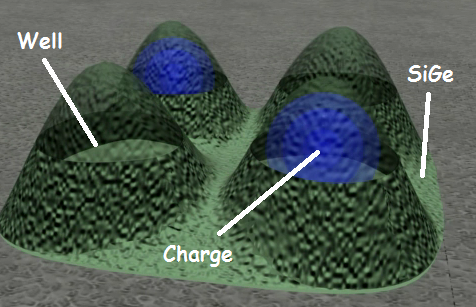
\includegraphics[width=\textwidth]{img/qca.png}
				\caption{QCA cells: physical view.}
		 	\end{figure} 
			\column{.5\textwidth}
			\begin{figure}
				\centering
				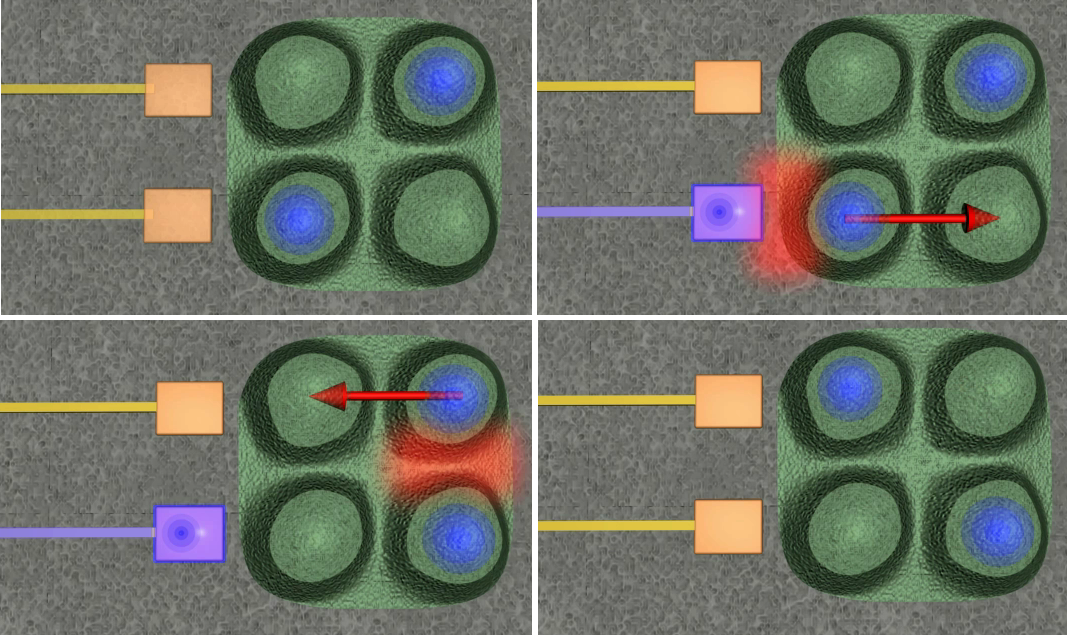
\includegraphics[width=\textwidth]{img/qcaevo.png}
				\caption{QCA cells: evolution of local state.}
			\end{figure}
		\end{columns}
		QCA are CA: evolution depends on previous status of cell itself and neighborhood
	\end{frame}

	\begin{frame}{The Problem}
	 	QCADesigner is slow... too slow
		\begin{itemize}
			\item A common MUX can take more than 4 hours to be simulated!
		\end{itemize}
		How to improve the performance of QCADesigner?
		\begin{itemize}
			\item Parallel programming on GPUs with Nvidia Cuda  
		\end{itemize}
	\end{frame}


\section{Nvidia Cuda}

	\begin{frame}{Cuda Overview}
		What is Cuda?		
		\begin{itemize}
			\item It is a software layer that allow programmers to exploit the capability of Nvidia GPUs as general purpose processors
		\end{itemize}
		Why Cuda for QCAD?
		\begin{itemize}
			\item Because GPUs offer parallelism and QCAs are parallel by nature
			\item Because GPUs are specialized in FP operations
			\item Because GPUs offer the lowest price per core
		\end{itemize}
	\end{frame}

	\begin{frame}{GPU Logical Organization and Programming Model}
		\begin{columns}
    		\column{.4\textwidth}
		 	\begin{figure}
				\centering
				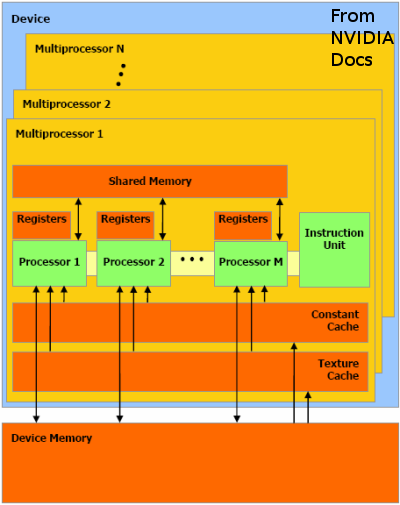
\includegraphics[width=\textwidth, height=0.6\textheight]{img/HWModel}
				\caption{Cuda GPUs: A MIMD Array of SIMD processors}
		 	\end{figure} 
			\column{.4\textwidth}
			\begin{figure}
				\centering
				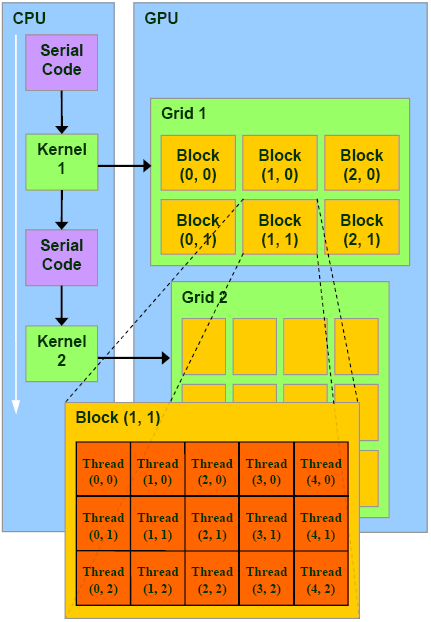
\includegraphics[width=\textwidth, height=0.6\textheight]{img/nVidiaExecutionModel}
				\caption{Cuda GPUs: Heterogeneous Programming}
			\end{figure}
		\end{columns}
	\end{frame}


\section{Implementation}

	\begin{frame}{Implementation Overview}
		\begin{columns}
			\column{.5\textwidth}
			QCADesigner
			\begin{itemize}
				\item Every cell - one thread approach
				\item Additive error when evolving system
				\item Time complexity: $O(2^i*n*b)$
			\end{itemize}
			\column{.5\textwidth}
			CudaQCADesigner
			\begin{itemize}
				\item One cell - one thread approach
				\item No additive error when evolving system
				\item Time complexity: $(\frac{2^i*n*b}{T})$ where $T$ is the number of running threads
			\end{itemize}
		\end{columns}
	\end{frame}

	\begin{frame}{Implementation}
		\begin{description}
			\item[QCADesigner] Every cell is simulated one after the other even though they could be evolved in parallel
			\item[CudaQCADesigner] Every thread is responsible for the evolution of its cell. The larger the number of running threads, the better the performances (upper bound: $T$=number of cells in the layout)
		\end{description}
	\end{frame}

	\begin{frame}{Implementation}
		choiches
	\end{frame}

\section{Results}

	\begin{frame}{Tests Description}
		The "Lucifero" Workstation
		\begin{description}
			\item[CPU] Intel Xeon E5345
			\item[GPU] Nvidia Testa C1060
		\end{description}
		Which Tests?
		\begin{description}
			\item[Test 1] QCAD vs CudaQCAD
			\item[Test 2] CudaQCAD Profiling
		\end{description}
	\end{frame}

	\begin{frame}{Test 1: QCAD vs CudaQCAD}
	 	\begin{figure}
			\centering
			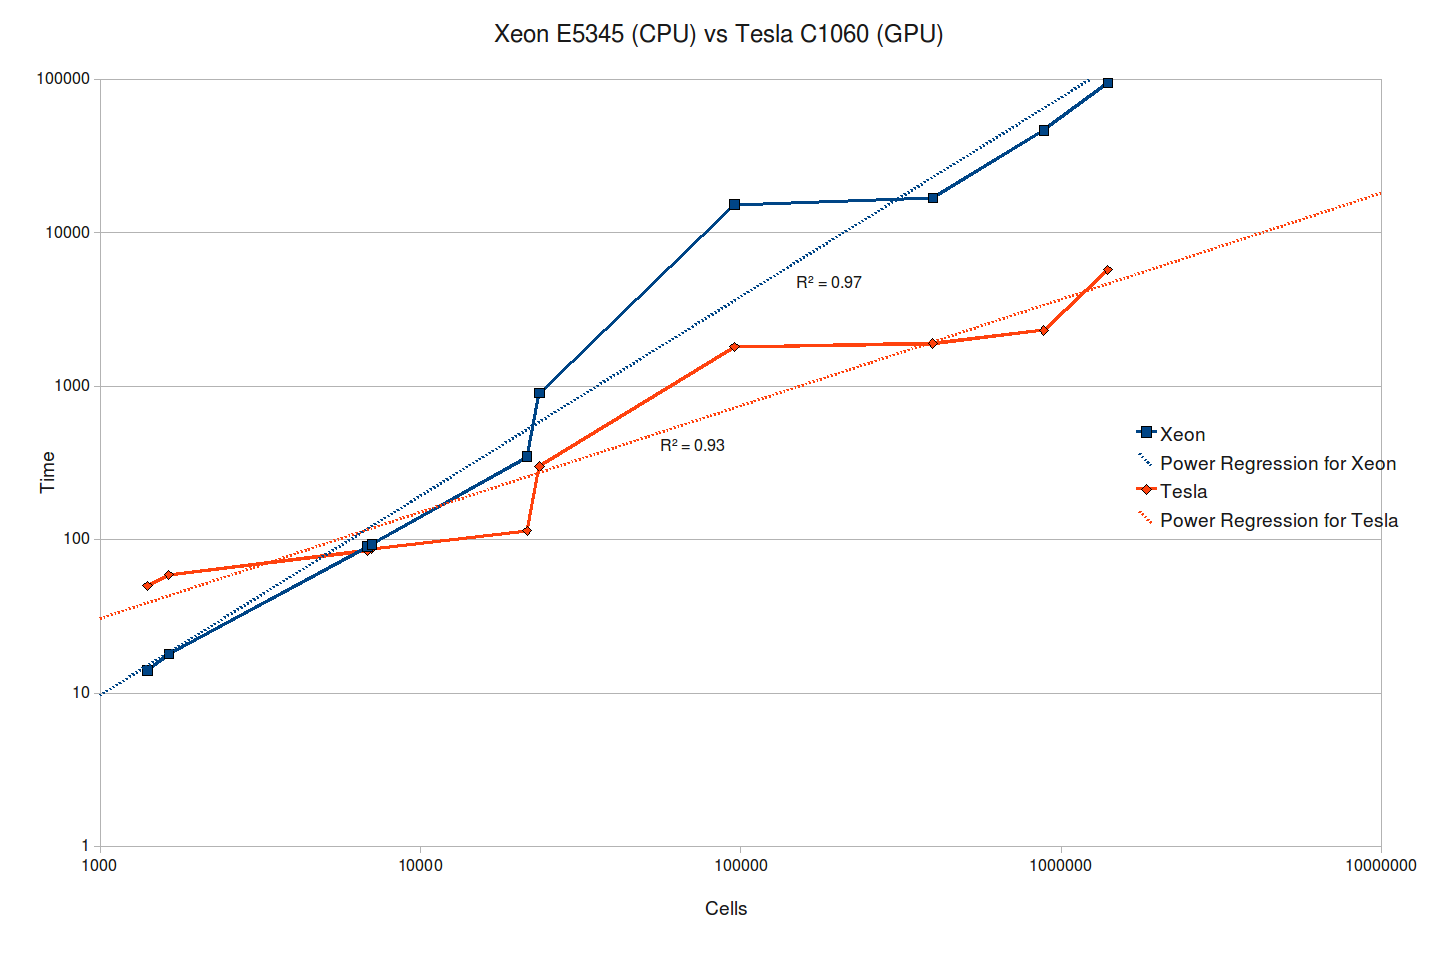
\includegraphics[width=\textwidth]{img/xeonvstesla}
	 	\end{figure} 
	\end{frame}

	\begin{frame}{Test 1: QCAD vs CudaQCAD}
	 	\begin{figure}
			\centering
			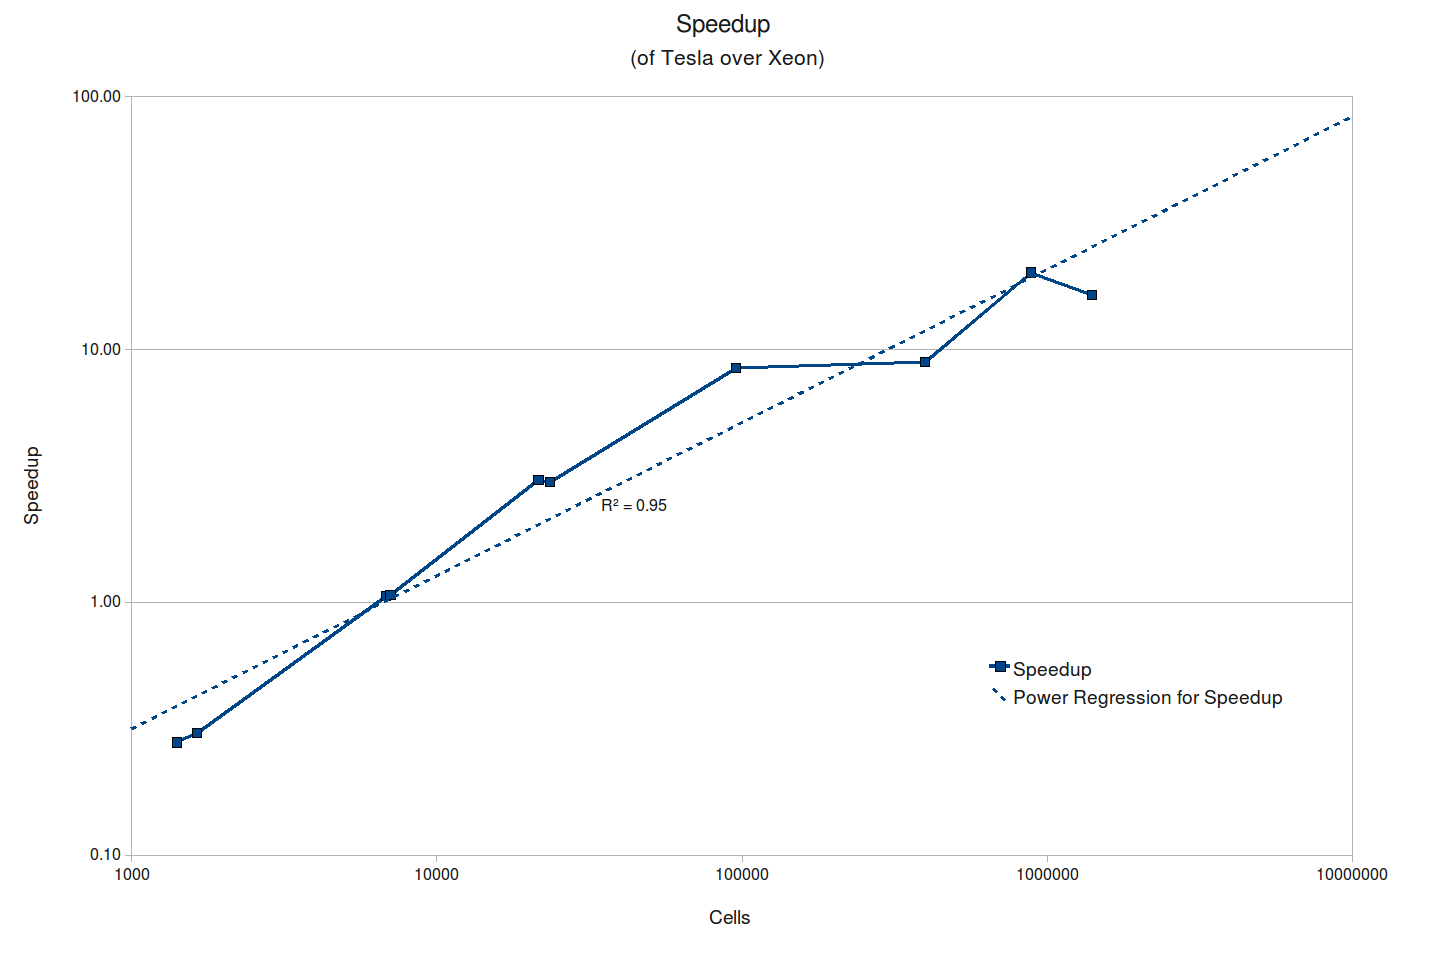
\includegraphics[width=\textwidth]{img/speedup}
	 	\end{figure} 
	\end{frame}

	\begin{frame}{Test 2: CudaQCAD Profiling - Memory Transfert Rate}
	 	\begin{figure}
			\centering
			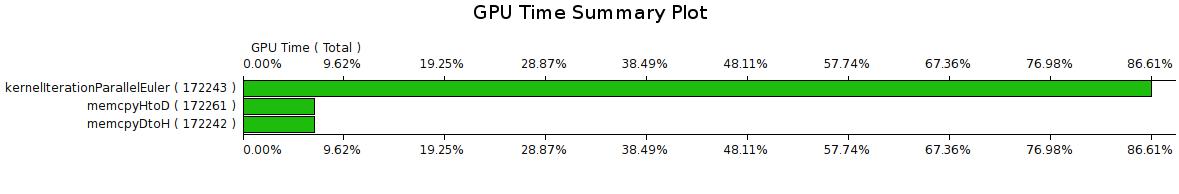
\includegraphics[width=\textwidth]{img/GPUTimeSummaryPlotNAND}
			\caption{Memory Tranfer for NAND circuit (1642 cells)}
	 	\end{figure} 
		\begin{figure}
			\centering
			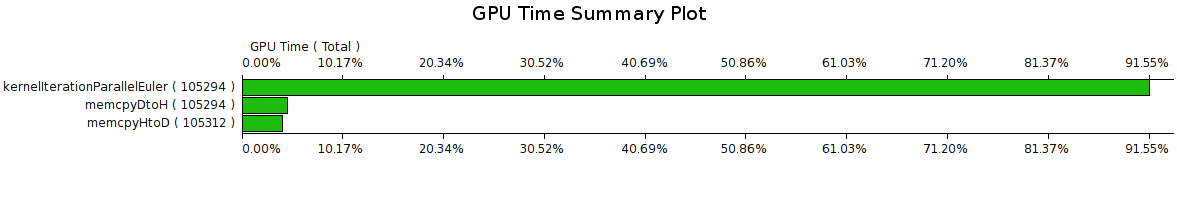
\includegraphics[width=\textwidth]{img/GPUTimeSummaryPlotMUX42}
			\caption{Memory transfers for MUX42 circuit (21551 cells)}
		\end{figure}
	\end{frame}

	\begin{frame}{Test 2: CudaQCAD Profiling - GPU Occupancy}
	 	\begin{figure}
			\centering
			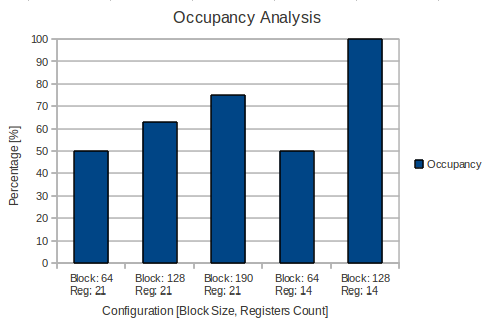
\includegraphics[width=\textwidth]{img/OccupancyAnalysis}
	 	\end{figure} 
	\end{frame}

	\begin{frame}{Conclusions}
		OBJ 1: Design a QCA simulator faster than QCADesigner
		\begin{itemize}
			\item CudaQCADesigner can significantly outperform QCADesigner for big circuits
		\end{itemize}
		OBJ 2: Produce a good Software
		\begin{itemize}
			\item CudaQCADesigner well exploits GPU resources
		\end{itemize}
	\end{frame}

	\begin{frame}{Questions?}
		\begin{columns}
		\column{.2\textwidth} 
			\textbf{Questions?}
		\end{columns}
	\end{frame}


\end{document}
